%% -*- coding: utf-8 -*-
\documentclass[12pt,a4paper]{report}
\usepackage[left=2cm,right=2cm,
    top=2cm,bottom=2cm,bindingoffset=0cm]{geometry} 
\usepackage[utf8]{inputenc}
\usepackage[english,russian]{babel}
\usepackage{indentfirst}
\usepackage{misccorr}
\usepackage{graphicx}
\usepackage{amsmath}
\usepackage{amsfonts}
\usepackage{amssymb}
\setcounter{page}{2}
\begin{document}

\begin{titlepage}
\newpage
  \begin{center}
     
    Санкт-Петербургский Политехнический Университет Петра Великого \\
    
    Институт компьютерных наук и технологий \\
    
    Кафедра компьютерных систем и программных технологий
    \end{center}
    
    \vspace{15em}
    \begin{center}
    \textsc{Лабораторная работа №7}\\
    \vspace{5mm}
    \textsc{Помехоустойчивое кодирование}
    	
   \end{center}
\vspace{10em}

\newlength{\ML}
\settowidth{\ML}{«\underline{\hspace{0.7cm}}» \underline{\hspace{2cm}}}
\hfill\begin{minipage}{0.45\textwidth}
\vfill
  Руководитель \\
  \\
  \underline{\hspace{\ML}} Богач Н.\,В.\\
 
\end{minipage}%
\bigskip

\hfill\begin{minipage}{0.45\textwidth}
  Выполнил\\
  \\
  \underline{\hspace{\ML}} Солдатова Е.\,И.\\
  группа 33501/3
\end{minipage}%

\vspace{\fill}
\begin{center}
    
  Санкт-Петербург\\
   2018 
\end{center}
\end{titlepage}

\paragraph{1. Цель работы\\\\}
Изучение методов помехоустойчивого кодирования и сравне-
ние их свойств

\paragraph{2. Постановка задачи\\}
\begin{enumerate}
\item Провести кодирование/декодирование сигнала, полученного с
помощью функции randerr кодом Хэмминга 2-мя способами: с
помощью встроенных функций encode/decode, а также через
создание проверочной и генераторной матриц и вычисление
синдрома. Оценить корректирующую способность кода.
\item Выполнить кодирование/декодирование циклическим кодом,
кодом БЧХ, кодом Рида-Соломона. Оценить корректирующую
способность кода.
\end{enumerate}

\paragraph{3. Теоретическая часть \\\\}
Кодированием и декодированием (в широком смысле) называют любое преобразование сообщения в сигнал и обратно, сигнала в сообщение, путем установления взаимного соответствия. Преобразование следует считать оптимальным, если в конечном итоге производительность источника и пропускная способность канала окажутся равными, т.е. возможности канала будут полностью использованы. Данное преобразование разбивается на два этапа:
\begin{itemize}
\item модуляция-демодуляция, позволяющая осуществить переход от непрерывного сигнала радиоканала к дискретному;
\item кодирование-декодирование (в узком смысле), во время которого все операции выполняются над последовательностью символов.
\end{itemize}

В свою очередь, кодирование-декодирование делится на два противоположных по своим действиям действиям этапа:
\begin{itemize}
\item устранение избыточности в принимаемом от источника сигнале (экономное кодирование);
\item внесение избыточности в передаваемый по каналу цифровой сигнал (помехоустойчивое или избыточное кодирование) для повышения достоверности передаваемой информации.
\end{itemize}

Циклический код — линейный, блочный код, обладающий свойством цикличности, то есть каждая циклическая перестановка кодового слова также является кодовым словом. Используется для преобразования информации для защиты её от ошибок.

К циклическим кодам относятся коды Хэмминга, которые являются одним из немногочисленных примеров совершенных кодов. Они имеют кодовое расстояние d = 3 и исправляют все одиночные ошибки. Длина кода выбирается из условия $2^{n-k} - 1	= n$, которое имеет простой смысл: число различных ненулевых синдромов равно числу символов в кодовой последовательности. 

Среди циклических кодов широкое применение нашли коды Боуза-Чоудхури-Хоквингема (БЧХ). Можно показать, что для любых целых положительных чисел m и l < n/2 существует двоичный код БЧХ длины $n=2^m - 1$, с кодовым расстоянием d > 2l + 1. Для кодов БЧХ умеренной длины и ФМ при передаче символов можно добиться значительного выигрыша (4 дБ и более). Он достигается при скоростях (1/3 < k/n < 3/4). При очень высоких и очень низких скоростях выигрыш от кодирования существенно уменьшается.

Частным случаем БЧХ кодов являются коды Рида-Соломона, корректирующая способность которых, соответственно, ниже.

\paragraph{4. Ход работы \\\\}
Результат кодирования/декодирования кодом Хэмминга с использованием стандартных функций:\\\\
msg = [0 1 1 1]\\
code = encode(msg,7,4)\\
code(1) = not(code(1))\\
{dec,err} = decode(code,7,4)\\

Результат работы программы:
\begin{figure}[h!]
\center{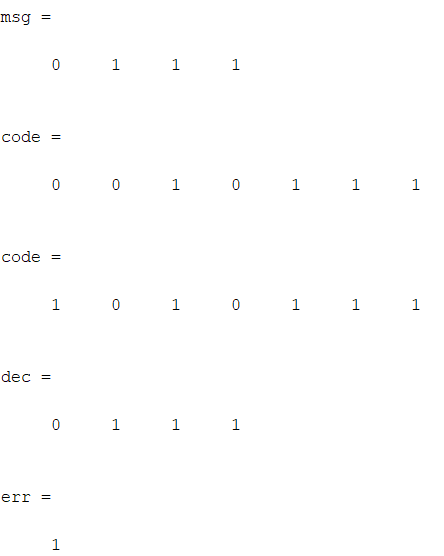
\includegraphics[width=0.4\linewidth]{1}}
\end{figure}

Результат кодирования/декодирования кодом Хэмминга с использованием проверочной и генераторной матриц и вычисление синдрома:\\\\
msg = [0 1 1 1]\\
{h,g,n,k} = hammgen(3)\\
m = msg*g;\\
m = rem(m,ones(1,n).*2);\\
m(4) = not(m(4));\\
synd = m*h';\\
synd = rem(synd,ones(1,n-k).*2);\\
stbl = syndtable(h);\\
tmp = bi2de(synd,'left-msb')\\
z = stbl(tmp+1,:)\\
rez = xor(m,z)\\
\newpage
Результат работы программы:
\begin{figure}[h!]
\center{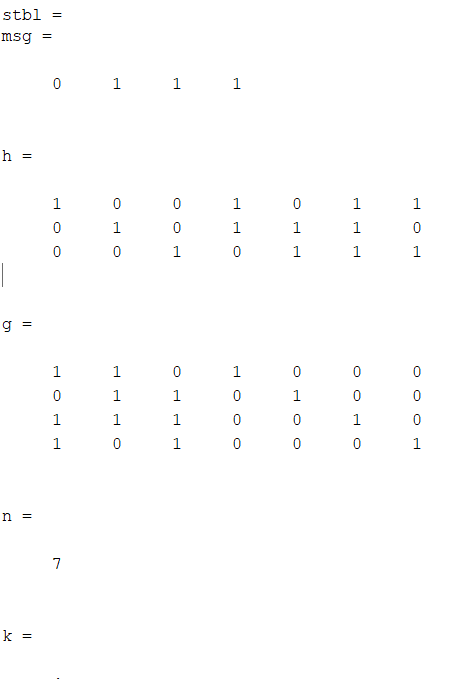
\includegraphics[width=0.4\linewidth]{2}}
\end{figure}
\begin{figure}[h!]
\center{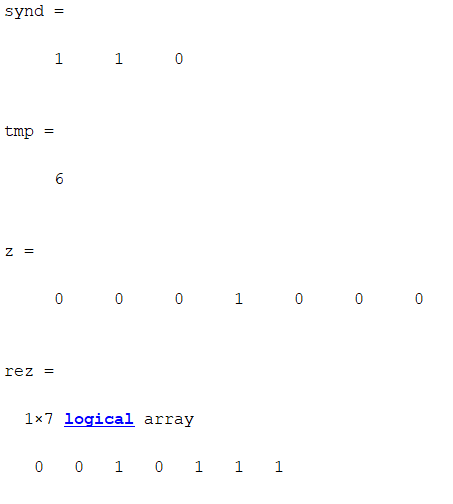
\includegraphics[width=0.4\linewidth]{3}}
\end{figure}

Результат кодирования/декодирования циклическим кодом:\\\\
msg = [0 1 1 1]\\
pol = cyclpoly(7,4)\\
{h,g} = cyclgen(7,pol);\\
code = msg*g;\\
code = rem(code,ones(1,n).*2);\\
code(2) = not(code(2));\\
synd = code*h';\\
synd = rem(synd,ones(1,n-k).*2);\\
stbl = syndtable(h);\\
tmp = bi2de(synd,'left-msb')\\
z = stbl(tmp+1,:)\\
rez = xor(code,z)\\

Результат работы программы:
\begin{figure}[h!]
\center{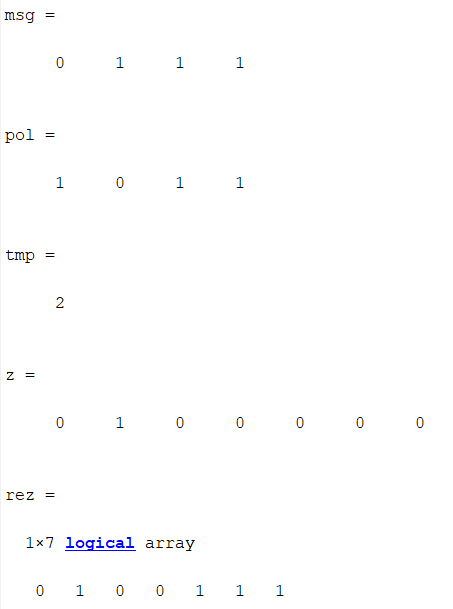
\includegraphics[width=0.4\linewidth]{4}}
\end{figure}

Результат кодирования/декодирования кодом БЧХ:\\\\
msg = [0 1 1 1]\\
codebch = comm.BCHEncoder(7,4)\\
decbch = comm.BCHDecoder(7,4)\\
temp = msg';\\
code = step (codebch , temp(:))'\\
code(2) = not(code(2))\\
decode = step (decbch , code')'\\
\newpage
Результат работы программы:
\begin{figure}[h!]
\center{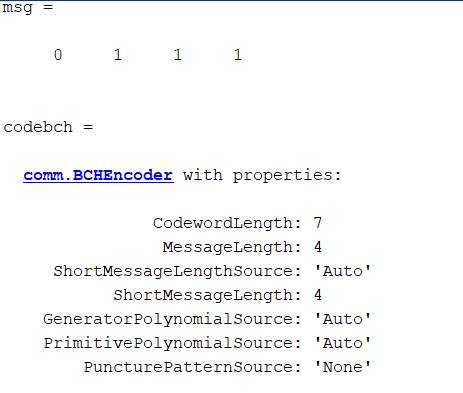
\includegraphics[width=0.4\linewidth]{5}}
\end{figure}
\begin{figure}[h!]
\center{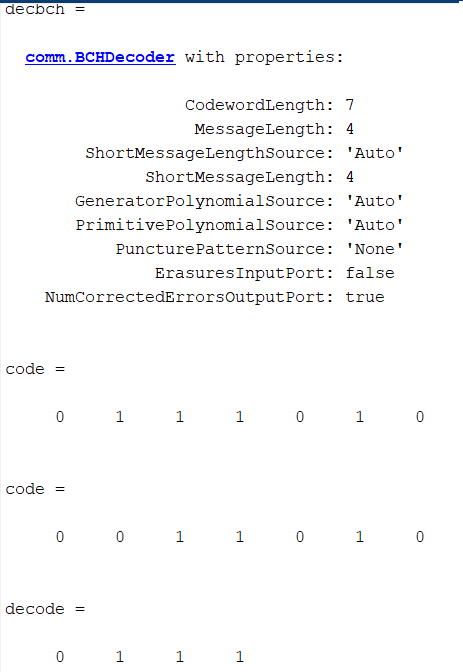
\includegraphics[width=0.4\linewidth]{6}}
\end{figure}

Результат кодирования/декодирования кодом Рида-Соломона:\\\\
m = 3;\\
n = 2\^m - 1;\\
k = 3;\\
msg = gf(0 1 2; 3 4 5; 6 7 6,m)\\
code = rsenc(msg,n,k)\\
errs = gf([0 0 0 4 0 0 0; 2 0 0 0 2 0 0; 3 4 5 0 0 0 0 ],m);\\
code = code + errs\\
dec,errnum = rsdec(code,n,k)\\
\newpage
Результат работы программы:
\begin{figure}[h!]
\center{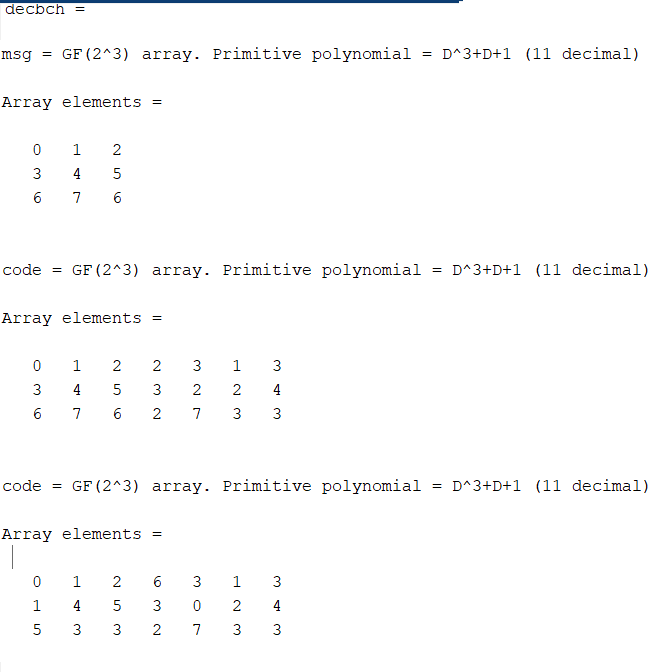
\includegraphics[width=0.4\linewidth]{7}}
\end{figure}
\begin{figure}[h!]
\center{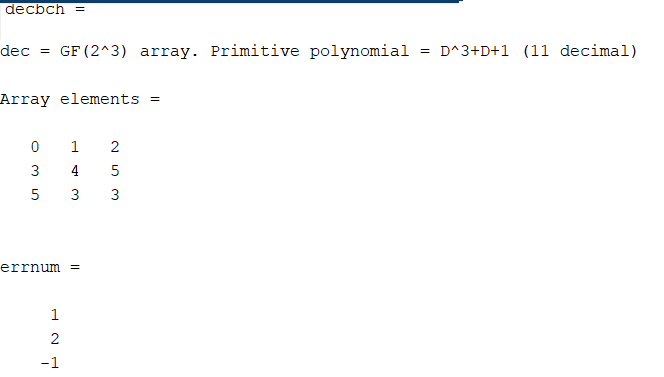
\includegraphics[width=0.4\linewidth]{8}}
\end{figure}

\paragraph{5. Выводы \\\\}
В ходе данной работы были получены навыки кодирования цифровых сигналов. Кодирование таких сигналов происходит по принципу избыточности. Каждый из исследованных кодов имеет свои преимущества и недостатки, поэтому использование конкретного из них должно быть обусловлено постановкой определенной задачи. Код Хэмминга достаточно простой в использовании, не требует больших мощностей. Однако он может исправить только одну допущенную ошибку в переданном сообщении. Код Рида-соломона способен исправлять несколько ошибок, так же он может оперировать десятичными числами, а не только двоичными.

\end{document}
